\documentclass{report}
\author{Ben Haladik}
\title{Bioinformatische Anwendung von \textit{Graphlets} zur Analyse von Proteinstrukturtopologien zur Analyse von Proteinen \\ Rohfassung}
\usepackage{mathtools}
\usepackage{amsfonts}
\usepackage{ngerman}
\usepackage{hyperref}
\usepackage{natbib}
%\usepackage{cite}

\begin{document}


\maketitle

\newpage

\tableofcontents

\newpage

\chapter{Einleitung}

\section{Motivation}

TODO: Zitationen einf\"ugen: schwierigkeit der Analyse, bereits bekannte Methoden

Dei \"Ahnlickeit von Proteinen zu bestimmen ist eine gro"se Herausforderung. In der Zeit als wenige Strukturen bekannt waren wurde die strukturelle \"Ahnlichkeit von Proteinen noch von Experten visuell bewertet, aber mittlerweile wurde die Strukturen von \"uber 100000 biologischen Makromolek\"ulen in der PDB. Der Vergleich dieser gigantischen Anzahl von Strukturdaten erfordert effiziente algorithmische Analysemethoden. Solche Analysen k\"onnen tiefe Einblicke in die ferne evolution\"are Verwandschaft von Proteinen liefern. Au"serdem sind sie im Bereich des \textit{Drug-Design} hoch interessant, denn  Strukturdaten liefer Informationen \"uber m \"ogliche Liganden, die ein Protein binden kann. Damit sind sie in der pharmakologischen Forschung von zentraler Bedeutung.
Das Problem hierbei ist, dass die Berechnung der \"Ahnlichkeit von 3D-Strukturen algorithmisch ein schwieriges Problem darstellt; lange Berechnungszeiten sind die Regel und es ist schwierig herauszufinden, ob der gefundene \"Ahnlichkeitswert f\"ur zwei Proteine nur ein lokales Optimum darstellt.
Deshalb wird versucht, von der 3D-Darstellung zu abstrahieren, ohne zentrale Strukturinformationen zu verlieren. Beispielsweise werden Distanzmatrizen verwendet, die die Abst\"ande einzelner Residuen zueinander speichern (DALI zitieren), anstatt die Koordinaten jedes Atoms abzuspeichern.
Auch Graphen eignen sich, um Strukturdaten in einer leichter zu analysierenden Form abzuspeichern. Denn Graphen k\"onnen genau wie Distanzmatrizen Informationen \"uber r\"aumliche N\"ahe aufbewahren.
Die PTGL \cite{ptgl1} speichert Proteinstrukturtopologien als Graphen ab. So werden zentrale Informationen \"uber die Struktur eines Proteins aufbewahrt w\"ahrend die Gr\"o"se der Daten ma"sgeblich reduziert wird. Diese Darstellung hat den weiteren Vorteil, dass Graphen zu den meistuntersuchten mathematischen strukturen der letzten Jahre geh\"oren. Soziale Netzwerke, Interaktionen von Proteinen in Zellen, das Internet: All diese Dinge lassen sich als Graphen darstellem und werden als solche untersucht.
Doch auch die \"Ahnlichkeit von Graphen zu bestimmen ist ein schwieriges Problem. Es gilt als NP-schwer (Zitat?).



\section{\textit{State of the Art}}

TODO: Methoden nennen, weitere Zitationen

Es gibt bereits einige Methoden, um Proteinstrukturen miteinander zu vergleichen. \textit{Hasegawa et al} \cite{advancespitfalls} liefern einen umfangreichen Vergleich verschiedener Methoden, bei denen Strukturen auf unterschiedlichen Abstraktionsstufen betrachtet und verglichen werden. So k\"onnen Proteinstrukturen dreidimensional, zweidimensional und eindimensional betrachtet und verglichen werden.

\paragraph{3D-Methoden} versuchen zun\"achst mittels Sequenzalignment einen Bereich in den zu vergleichenden Proteinen zu finden, in dem sich beide Proteine sehr \"ahnlich sind. Dieser Bereich fungiert gewisserma"sen als \emph{Anker} f\"ur das weitere Alignment. In den weiteren Schritten werden die Proteine so positioniert, dass die Distanzen in dem alignierten Bereich minimal sind. Von diesem \textit{Template} ausgehend, werden die Distanzen zwischen den weiteren Residuen der Proteine berechnet und meist mittels \textit{Root-mean-square-deviation} bewertet.

\paragraph{2D-methoden} versuchen Kontakte zwischen Residuen oder Sekund\"arstrukturen zu vergleichen. Diese Kontakte werden beispielsweise als graphen oder Distanzmatrizen dargestellt. Der Vergleich zwischen zwei Proteinstrukturen wird dann beispielsweise als Verlgeich zweier Distanzmatrizen durchgef\"uhrt.

\paragraph{1D-Methoden} nutzen Strukturprofile zur Darstellung von Proteinen. In Strukturprofilen repr\"asentieren einzelne Buchstaben Eigenschaften von Residuen und die Konformation des Protein-\textit{Backbone} an der entsprechenden Stelle. So k\"onnen schnelle \textit{String}-Algorithmen genutzt werden, um Strukturen zu suchen und zu vergleichen.

\paragraph{0D-Methoden} reduzieren die 3D-Struktur am st\"arksten. Die gesamte Struktur wird durch eine Zahl beschrieben, die sich aus der Struktur berechnen l\"asst. Sie erlauben sehr schnelle Suchen in Datenbanken, haben aber das Problem, dass sie keinen Vergleich von Teilstrukturen erm\"oglichen.

\paragraph{Die Methoden} stellen alle einen Versuch dar, die \"Ahnlichkeit von Proteinen zu beziffern. Sie werden angewendet, um entferent homologe Proteine aufzusp\"uren und in Datenbanken eine \"Ahnlichkeitssuche zu erm\"oglichen. Dies findet vor allem im pharmakologischen Bereich Anwendung.

Interessant ist, dass unter den von \textit{Hasegawa et al} vorgestellten 1D-Methoden keine wirklich analog zur Analyse mit \textit{Graphlets} funktioniert. Andere 1D-Methoden versuchen die Polypeptidkette als \textit{String} darzustellen und damit die Konformations\"anderung des \textit{Backbone} zu beschreiben. Im Gegensatz dazu z\"ahlt der \textit{Graphlet}-Algorithmus die \textit{Graphlets} unabh\"angig von ihrer Position im Graphen. Somit repr\"asentiert der \textit{Graphlet}-Vektor an jeder Stelle eine globale Eigenschaft des Graphen, anstatt die Ver\"anderung von einer Sekund\"arstruktur zur n\"achsten zu beschreiben.

\section{Ziele}

TODO: Zitationen einf\"ugen

Ziel der Arbeit war festzustellen, ob sich \textit{Graphlets} eignen, um \"Ahnlichkeiten von Proteinstrukturen festzustellen. In den Arbeiten von \emph{Hasegawa et al}, \emph{Pr\v{u}lj et al} und \emph{Shervashidze} wurden \textit{Graphlets} bereits erfolgreich angewandt, um die \"Ahnlichkeiten von Netzwerken zu bestimmen. Ihre analysen wurden haupts\"achlich f\"ur sehr gro"se netzwerke, wie PPI-Graphen und (siehe TODO, arbeit von Shervashidze) durchgef\"uhrt. Somit blieb die Frage offen, ob sich \textit{Graphlets} auch zur analyse von Netzwerken eigenen, die deutlich kleiner sind und deutlich niedrigere Knotengrade haben.
Weiterhin galt es, herauszufinden, welche Metriken sich am besten eignen, um die Unterschiede zwischen verschiedenen Topologien zu befiffern.
Hiermit k\"onnte schlie"slich eine \"Ahnlichkeitssuche in der PTGL implementiert werden.

\section{Aufbau der Arbeit}

Zun\"achst wird im Kapitel \emph{Materialien und Methoden} PLCC vorgestellt - das Programm, mit dem die Graphen der PTGL erzeugt werden. Es folgt eine Kurzbeschreibung der PTGL selbst, sowie eine Beschreibung des \textit{Graphlet}-Algorithmus. Weiterhin wird das Programm\texttt{graphletAnalyser}vorgestellt, welches den \textit{Graphlet}-Algorithmus implementiert. Es werden verschiedene Metriken vorgestellt und evaluiert, mit denen die erhaltenen \textit{Graphlet}-Vektoren verglichen werden.
Abschlie"send folgt eine kurze Beschreibung des FATCAT-SCOP-\textit{Benchmarking}-Datensatzes und der f\"ur die Fallstudien ausgew\"ahlten Proteine.
Die dabei erhaltenen Ergebnisse werden im gleichnamigen folgenden Kapitel vorgestellt. Eine Diskussion der Ergebnisse und ein Ausblick auf weitere Anwendungen und Verbesserungsm\"oglichkeiten erfolgt im letzten Kapitel.

\chapter{Materialien und Methoden}

Um die Proteinstrukturtopologien aus der PTGL zu vergleichen wurde das Programm \texttt{graphletAnalyser} genutzt und erweitert. Es wurde bereits 2013 von \textit{Tatiana Bakirova} im Rahmen ihrer Diplomarbeit im Arbeitskreis \textit{Molekulare Bioinformatik} geschrieben. Die urspr\"ungliche Funktionalität wurde erweitert. Hierbei wurden Funktionen zur Analyse von Komplexgraphen, Aminos\"auregraphen und den Sekund\"arstrukturgraphen implemetiert. Diese Graphen stammen allesamt aus der PTGL (\underline{P}rotein \underline{T}opology \underline{G}raph \underline{L}ibrary) von Tim Sch\"afer.

\section{PLCC}

\section{Die PTGL}


Die \underline{P}rotein \underline{T}opology \underline{G}raph \underline{L}ibrary ist 2009 von \textit{May et al.} \cite{ptgl1} entwickelt worden. Sie stellt ein System zur Klassifizierung von 3D Proteinstrukturen zur Verf\"ugung. Es gibt berei


\section{Der \textit{Graphlet}-Algorithmus}

\paragraph{Motivation}
Die PTGL \cite{vplg} erm\"oglicht also die Darstellung von Proteinstrukturtopologien als Graphen. Um aus diesen Graphen weitere Informationen zu gewinnen, ist es sinnvoll, sie untereinander vergleichen zu k\"onnen. Ein solcher Vergleich ist jedoch ein schwieriges Problem: Gesucht ist eine Funktion $f: (G,G') \rightarrow \mathbb{R} $, die f\"ur zwei Graphen $G$ und $G'$ deren \"Ahnlichkeit zueinander beziffert.
Es gibt diverse M\"oglichkeiten diesesd Problem zu bearbeiten, von denen jedoch keine einfach ist.
Eine M\"oglichkeit ist, die Suche nach gr\"o"sten gemeinsamen isomorphen Teilgraphen in $G$ und $G'$, oder man versucht eine Editierdistanz zu berechnen - also herauszufinden, wie viele Operationen (Hinzuf\"ugen oder Entfernen von Knoten und Kanten) n\"otig sind um $G$ in $G'$ zu \"uberf\"uhren. Diese beiden genannten Methoden erfordern jedoch aufw\"andige Berechnungen.
Deshalb werden Methoden verwendet, die \emph{Topologische Charakteristiken} berechnen und dies in polynomieller Laufzeit bewerkstelligen. Der Vorteil hierbei ist, dass die (aufw\"andige) Berechnung dieser Charakteristiken nur einmal pro Graph erfolgen muss. Die Charakteristiken k\"onen dann als Datenpunkte verglichen werden und man spart sich die Berechnungen, die man sonst f\"ur alle Paare von Graphen $G,G'$ durchf\"uhren muss.
Eine Algorithmus, mit dem sich solche Charakteristiken verechnen lassen wurde 2009 von \textit{N. Shervashidze} vorgestellt: Der \textit{Graphlet}-Algorithmus.


\paragraph{Beschreibung des Algorithmus}
\textit{Graphlets} sind kleine induzierte Teilgraphen eines gr\"o"seren ungerichteten Graphen. \textit{N. Shervashidze} stellte diese Methode als Vergleichsschema f\"ur Graphen 2009 zum ersten Mal vor.  (Literaturverweis einf\"ugen). Folgendes Bild zeigt alle \textit{Graphlets} der Gr\"o"se 4:

\begin{figure}[h]
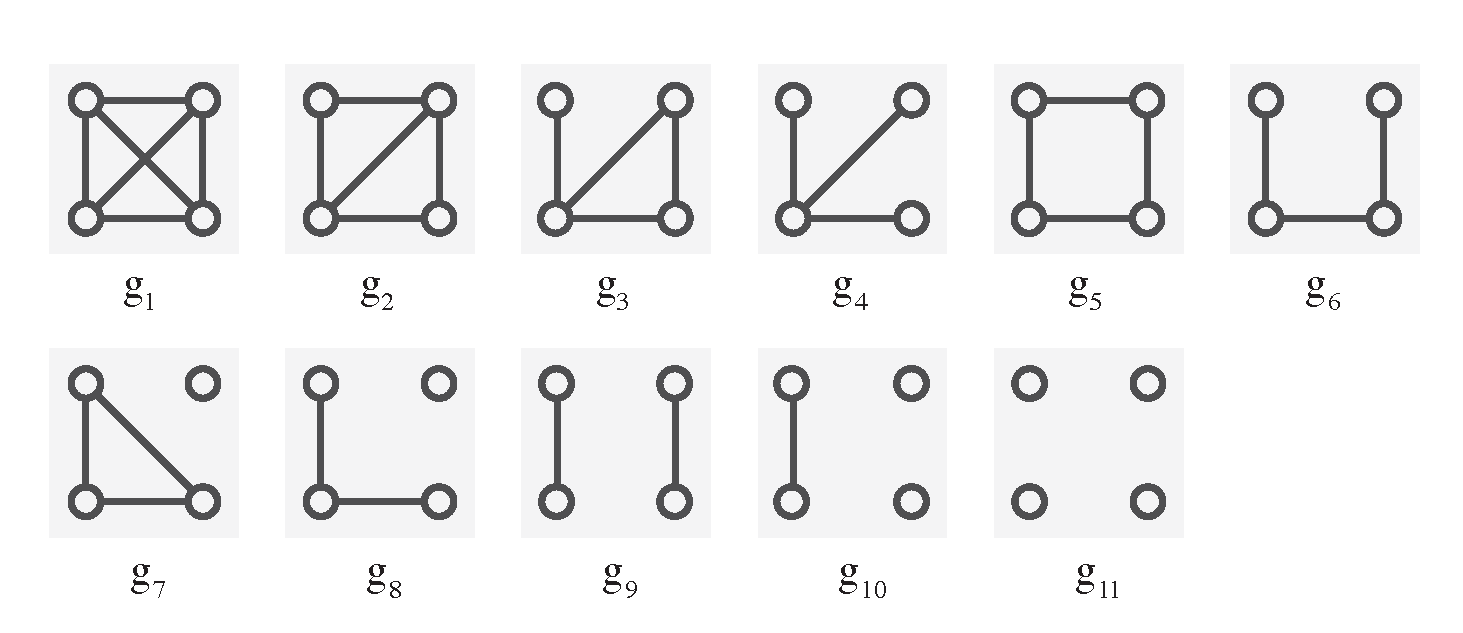
\includegraphics[width =\linewidth]{4graphlets.pdf}
\caption{Graphlets der Gr\"o"se 4 (\textit{Shervashidze et al.})}
\label{fig:4graphlets}
\end{figure}


Um ein \textit{Graphlet} der Gr\"o"se k zu finden, besucht der Algorithmus alle Euler-Wege der L\"ange k, in dem gegebenen Graphen. F\"ur jeden dieser Wege \"uperpr\"uft er, f\"ur alle Paare von Knoten $v,w$ ob es eine Kante $e = {v,w}$ gibt, die nicht zu dem besuchten Euler-Weges gehg\"ort. Je nachdem, welche Kanten hierbei gefunden werden, wird der Z\"ahler f\"ur das entsprechende \textit{Graphlet} erh\"oht. Der Algorithmus z\"ahlt hier aber nur alle zusammenh\"angenden \textit{Graphlets}. Er verwendet die folgenden Gewichtungsvektoren: 


\begin{subequations}
\label{eq:w-vector}
\textit{Graphlet}-Gewichtungsvektoren
\begin{align}
w_2 := \left( \frac{1}{2} \right) \\
w_3 := \left( \frac{1}{6}, \frac{1}{2} \right) \\
w_4 := \left( \frac{1}{24}, \frac{1}{12}, \frac{1}{4}, 1, \frac{1}{8},\frac{1}{2} \right) \\
w_5 := \left( \frac{1}{120}, \frac{1}{72}, \frac{1}{48}, \frac{1}{36}, \frac{1}{28}, \frac{1}{20}, \frac{1}{14}, \frac{1}{10}, \frac{1}{12}, \frac{1}{8}, \frac{1}{4}, \frac{1}{2}, \frac{1}{12} \frac{1}{12}, \frac{1}{4} \frac{1}{4}, \frac{1}{2}, 1, \frac{1}{2}, 1\right)
\end{align}
\end{subequations}

Jede Stelle eines Vektors $w_i$ ist mit einem \textit{Graphlet} assoziiert. Da der Algorithmus alle Euler-Wege einer L\"ange $i$ in dem Graphen abl\"auft, sind in den Vektoren Br\"uche eingetragen, wobei der Z\"ahler f\"ur die Anzahl der Euler-Wege der L\"ange $i$ steht. Dies stimmt nat\"urlich nicht f\"ur die sogenannten Stern-\textit{Graphlets} ($g_4$ in \ref{fig:4graphlets} $g_{19}$,$g_{20}$ und $g_{21}$ in \ref{fig:5graphlets}). Da diese keinen Euler-Weg der L\"ange 4 bzw. 5 enthalten werden sie anders gez\"ahlt.
(beispiel mit Pseudocode einf\"ugen?)


\section{\texttt{graphletAnalyser}}

Der \texttt{graphletAnalyser} berechnet die oben beschreibenen \textit{Graphlets} nach dem Algorithmus von \emph{Shervashidze et al.}. ZUr Zeit unterst\"utzt er die Berechnung f\"ur 3 verschiedene Graphen der PTGL: 
SSE-Graphen sind Graphen, die eine Polypeptidkette als Graph darstellen indem sie ihre Sekund\"arstrukturelemente als Knoten repr\"asentieren und diese mit Kanten verbinden, wenn sie r\"aumlich benachbart sind. \\
Komplexgraphen sind Graphen f\"ur Proteinkomplexe; sie modellieren mehrere Polypeptidketten indem sie mehrere SSE-Graphen miteinander verkn\"upfen. \\
Aminos\"auregraphen modellieren einzelne Aminos\"auren als Knoten und verbinden diese miteinander, wenn sie r\"aumlich benachbart sind. Dementsprechend ein Vielfaches der Knoten und Kanten eines SSE- oder Komplex-Graphen. \\
Zus\"atzlich zu den \textit{Graphlets} bis zur Gr\"o"se 5 berechnet das Programm markierte \textit{Graphlets} mit bis zu 3 Knoten. Dabei werden zun\"achst alle Markierungen die kombinatorisch m\"oglich sind berechnet und die entsprechenden \textit{Graphlets} werden gez\"ahlt.\\
Das Programm wird \"uber die Kommandozeile aufgerufen und erh\"alt eine oder mehrere GML-Dateien als Argumente.
Zus\"atzlich kann angegeben werden, ob die GML-Datei einen Proteingraphen, Komplexgraphen oder Aminos\"auregraphen beschreibt.
Alternativ kann auch in der Konfigurationsdatei angegeben werden, dass eine andere Art von Graph eingelesen werden soll.
\texttt{graphletAnalyser} ist also in der Lage, jede GML-Datei, die einen ungerichteten Graphen enth\"alt einzulesen und f\"ur sie \textit{Graphlets} zu berechnen. Der Nutzer kann weiterhin ein Alphabet unterschiedlicher Knotenmarkierungen angeben, f\"ur das markierte \textit{Graphlets} berechnet werden. Somit kann das Programm auch f\"ur graphenbezogene Fragestellungen verwendet werden, die sich nicht auf Proteine beziehen.
Aus der .gml-Datei wird ein Graph erstellt. Das Programm nutzt hierbei die \textit{Boost-Graph-Library} zur internen Darstellung. Entsprechend der vom Nutzer ausgew\"ahlten Funktionen werden die \textit{Graphlets} berechnet und als Datei ausgegeben. Zus\"atzlich k\"onnen sie in einer lokalen Datenbank abgespeichert werden.


\section{Scoring}



\subsection{Tanimoto-Koeffizient}

\subsection{Relative \textit{Graphlet}-H\"aufigkeiten-Distanz}

\textit{N. Pr\v{z}ulj et al.} haben \textit{Graphlets} bereits in verschiedensten Zusammenh\"anen auf biologische Daten wie Protein-Protein-Interaktionsnetzwerke \cite{frqdistribution} angewandt. Als Ma"s f\"ur die \"Ahnlichkeit von Netzwerken nutzen sie die Relative-\textit{Graphlet}-H\"aufigkeiten-Distanz $D(G,H)$. Diese Metrik bestimmt den Unterschied zwischen zwei Graphen $G$ und $H$ als logarithmierte Differenz der normalisierten Anzahl der \textit{Graphlets} in $G$ und $H$. Sie ist folgenderma"sen definiert: \\

Sei $N_{i}(G)$ die Anzahl der \textit{Graphlets} von Typ $i \in {1,...,29}$ und \\ $T(G) = \sum_{i = 1}^{29} N_{i}(G)$ die Anzahl der \textit{Graphlets} in $G$, beziehungsweise $H$\\

Dann ist die Relative-\textit{Graphlet}-H\"aufigkeiten-Distanz $D(G,H)$ f\"ur zwei Graphen $G$ und $H$ definert als:

\begin{subequations}
\begin{align}
D(G,H) = \sum_{i = 1}^{29} | F_{i}(G) - F_{i}(H) | \\
mit F_{i}(G) = - log(\frac{N_{i}(G)}{T(G)})
\end{align}
\end{subequations}



Diese Metrik hat den Vorteil, dass sie die normailisierten \textit{Graphlet}-Vektoren verwendet. So ist ein guter Vergleich auch m\"oglich, wenn einzelne \textit{Graphlets} in den Netzwerken \"uberrepr\"asentiert sind.
Weiterhin wurde gezeigt, \cite{frqdistribution} dass diese Metrik auch bei verrauschten Daten noch sehr gut funktioniert.

\subsection{\textit{Root-Mean-Square-Deviation}}

Die \textit{Root-Mean-Square-Deviation} RMSD ist ein Standardma"s zur Abstandsmessung in Vektorr\"aumen. Sie wird f\"ur zwei Vektoren $x$ und $y$ durch folgende Formel berechnet:

\begin{subequations}
\label{eq:rmsd}
\begin{align}
RMSD = \sum_{i=1}^{n} (x_i - y_i)^2
\end{align}
\end{subequations}


\section{Datens\"atze}


\subsection{FATCAT-SCOP-\textit{Benchmarking-Set}}

Die FATCAT SCOP DB, beschrieben in: http://bioinformatics.oxfordjournals.org/content/23/2/e219.long
k\"onnte sich gut zum Vergleich eignen

Das FATCAT-SCOP-\textit{Benchmarking-Set} ist f\"ur das Strukturalignment-Programm FATCAT \cite{fatcat} zusammengestellt worden, um seine Performance mit der von etablierten Strukturalignment-Programmen wie DALI und CE zu vergleichen. Der Datensatz besteht aus 2256 PDB-Eintr\"agen, die bereits durch die SCOP-Datenbank klassifiziert worden sind.
In dem Datensatz befinden sich Paare von PDB-Eintr\"agen, die von allen drei Programmen als sehr \"ahnlich bewertet wurden. 


\subsection{Fallstudien}


\subsubsection{4-Helix-\textit{Bundles}}

Das Cytochrom B562 von \emph{E. coli} (Bild einf\"ugen) ist ein Protein, das f\"ur Elektronentransport zust\"andig ist. Strukturell wird es als 4-Helix-\textit{Bundle} eingeordnet. Zu diesem Protein gibt es zwei PDB-Eintr\"age: 1QPU und 256B. Es gibt von diesem Rrotein auch eine Hem-bindende Variante, die oxidiert ist. Sie hat die PDB-ID 1QQ3. All diese Strukturdaten werden von CATH als sehr \"ahnliche Strukturen mit hoher Sequenzidentit\"at eingeordnet.
Um die Parameter und Metriken f\"ur den Vergleich zu testen, bietet es sich an, diese Proteine mit weiteren Proteinen aus der selben homologen Superfamilie zu vergleichen und diese dann mit Proteinen aus anderen Homologen Superfamilien zu vergleichen. Die entsprechenden Proteine werden h\"andisch entsprechend der Einordnung durch CATH gew\"ahlt. Proteine die neu designt wurden k\"onnten sich auch anbieten. Inwiefern eine Untersuchung an ihnen sinnvoll ist, muss aber noch \"uberpr\"uft werden.
Weitere PRoteine aus der Homologen Superfamilie, die sich eignen sind:\\
2XL6: Cytochrom C aus Alcaligenes Xylosoxidans, gebunden mit NO\\
2YL1: s.o. nur andere Variante mit anderem Bindungspartner.\\
Diese beiden m\"ussten strukturell \"ahnlicher sein, als die weiter oben genannten Varianten von Cytochrom B562.\\
Die oben genannten Proteine werden von CATH alle in die \emph{Topologie} der 4-Helix-\textit{Bundles} (Hemerythrin Untereinheit A) eingeordnet.




\subsubsection{Wachstumshormone}

Sie k\"onnen mit Proteinen aus der Topologie \textit{Growth Hormone, Chain A} verglichen werden. Denn beide werden von CATH in die gleiche Architektur \emph{Up-down bundle} eingeordnet. Proteine aus dieser Topologie sind: \\
1HGU: Menschliches Wachstumshormon\\
1M4R: Rekombinantes menschliches Interleukin 22\\
1D9C: Rinder Interferon Gamma \\
Die oben genannten Proteine aus der Topologie der Wachstumshormone haben eine Sequenzidentit\"at zwischen 35 und 60 Prozent. Sie scheinen sich gut f\"ur die untersuchung zu eignen.

\subsubsection{Aldolasen}

Die Aldolasen 7TIM, 1NEY und 2V5L werden durch das gleich Gen in Hefe codiert. Da sie eine $\beta$-\textit{Barrel}-Struktur besitzen, sollten sie eine niedrigere \textit{Graphlet}-Distanz zueinander aufweisen, als zu allen anderen Strukturen.

\subsubsection{Zusammengefasst}

\begin{tabular}{l r}

PDB-ID & CATH-Code  \\
1QPU & 1.20.120.10  \\
1QQ3 & 1.20.120.10  \\
2XL6 & 1.20.120.10  \\
2YL1 & 1.20.120.10  \\
1HGU & 1.20.1250.10 \\
1M4R & 1.20.1250.10 \\
1D9C & 1.20.1250.10 \\
7TIM & 3.20.20.70   \\
1NEY & 3.20.20.70   \\
2V5L & 3.20.20.70   \\

\end{tabular}



\chapter{Ergebnisse}


\section{Fallstudie - vergleich mit Dali}




\chapter{Diskussion und Ausblick}





Es bieten sich Paper an, die in Liisa Holm \textit{Advances and Pitfalls of Protein Structure Prediction} besprochen wurden. Das Problem ist, dass \texttt{graphletAnalyser} Vektoren erzeugt - also eindimensionale Daten. Somit eignen sich Methoden, die 2D- oder 3D-Daten miteinander alignieren schlecht zum Vergleich. \textit{Holm} erw\"ahnt in ihrer Arbeit aber auch Autoren, die Vergleiche von eindimensionalen Daten durchgef\"uhrt haben. Dies sind folgende:

Liu X, Zhao YP, Zheng WM: CLEMAPS: multiple alignment of protein structures based on conformational letters

Sierk ML, Pearson WR: Sensitivity and selectivity in protein structure comparison

Sacan A, Toroslu IH, Ferhatosmanoglu H: Integrated search and alignment of protein structures

Friedberg I, Harder T, Kolodny R et al. Using an alignment of fragment strings for comparing protein structures

Tung CH, Huan JW, Yang JM: Kappa-alpha plot derived structural alphabet and BLOSUM-like substitution matrix for rapid search of protein structure database






Yang JA: Comprehensive description of protein structures using protein shape code




\chapter{Anhang}

\section{Tabellenverzeichnis}

\section{Bildverzeichnis}

\begin{figure}[h]
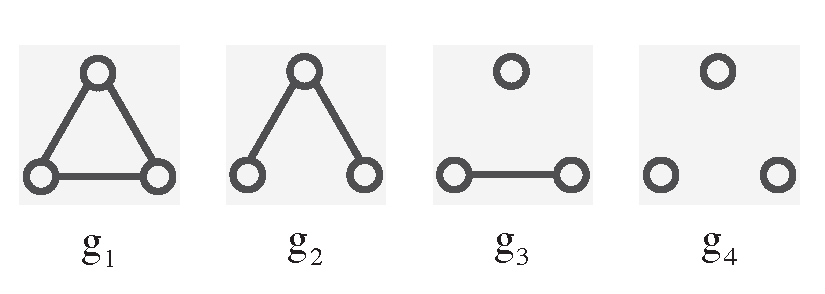
\includegraphics[width =\linewidth]{3graphlets.pdf}
\caption{Graphlets der Gr\"o"se 3 (\textit{Shervashidze et al.})}
\label{fig:3graphlets}
\end{figure}

\begin{figure}[h]
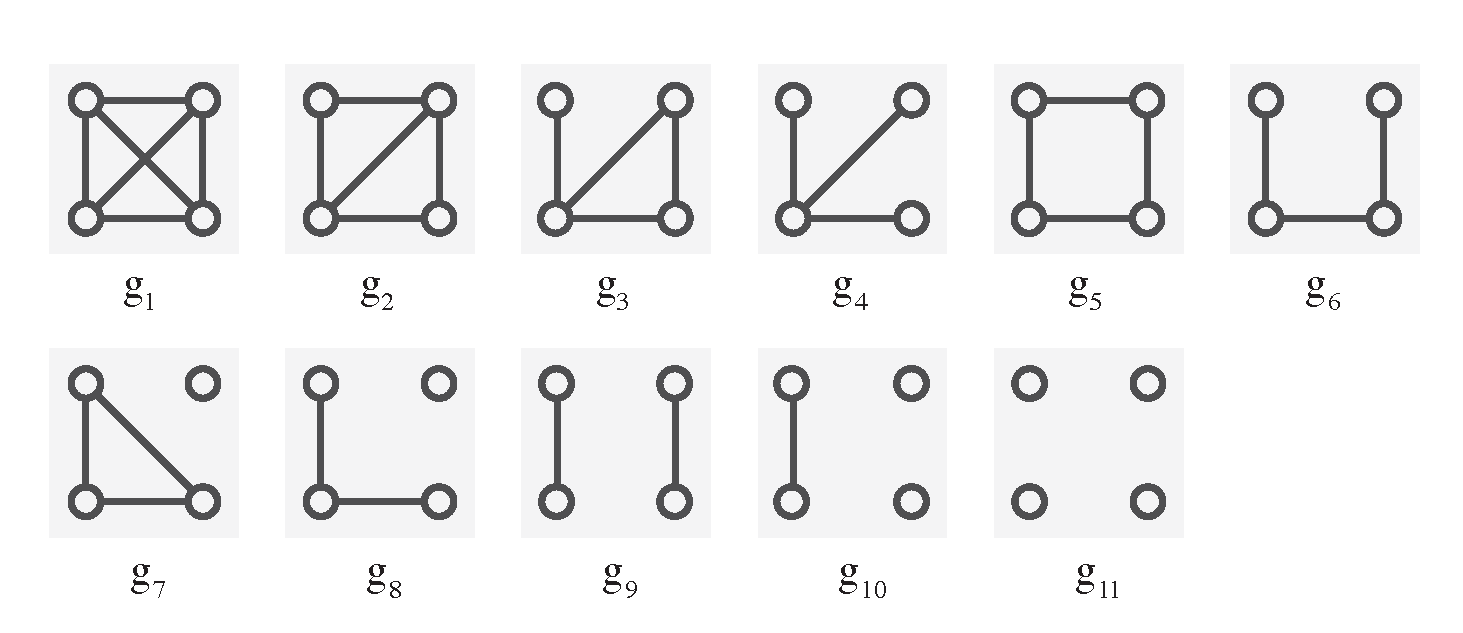
\includegraphics[width =\linewidth]{4graphlets.pdf}
\caption{Graphlets der Gr\"o"se 4 (\textit{Shervashidze et al.})}
\label{fig:4graphlets2}
\end{figure}

\begin{figure}[h]
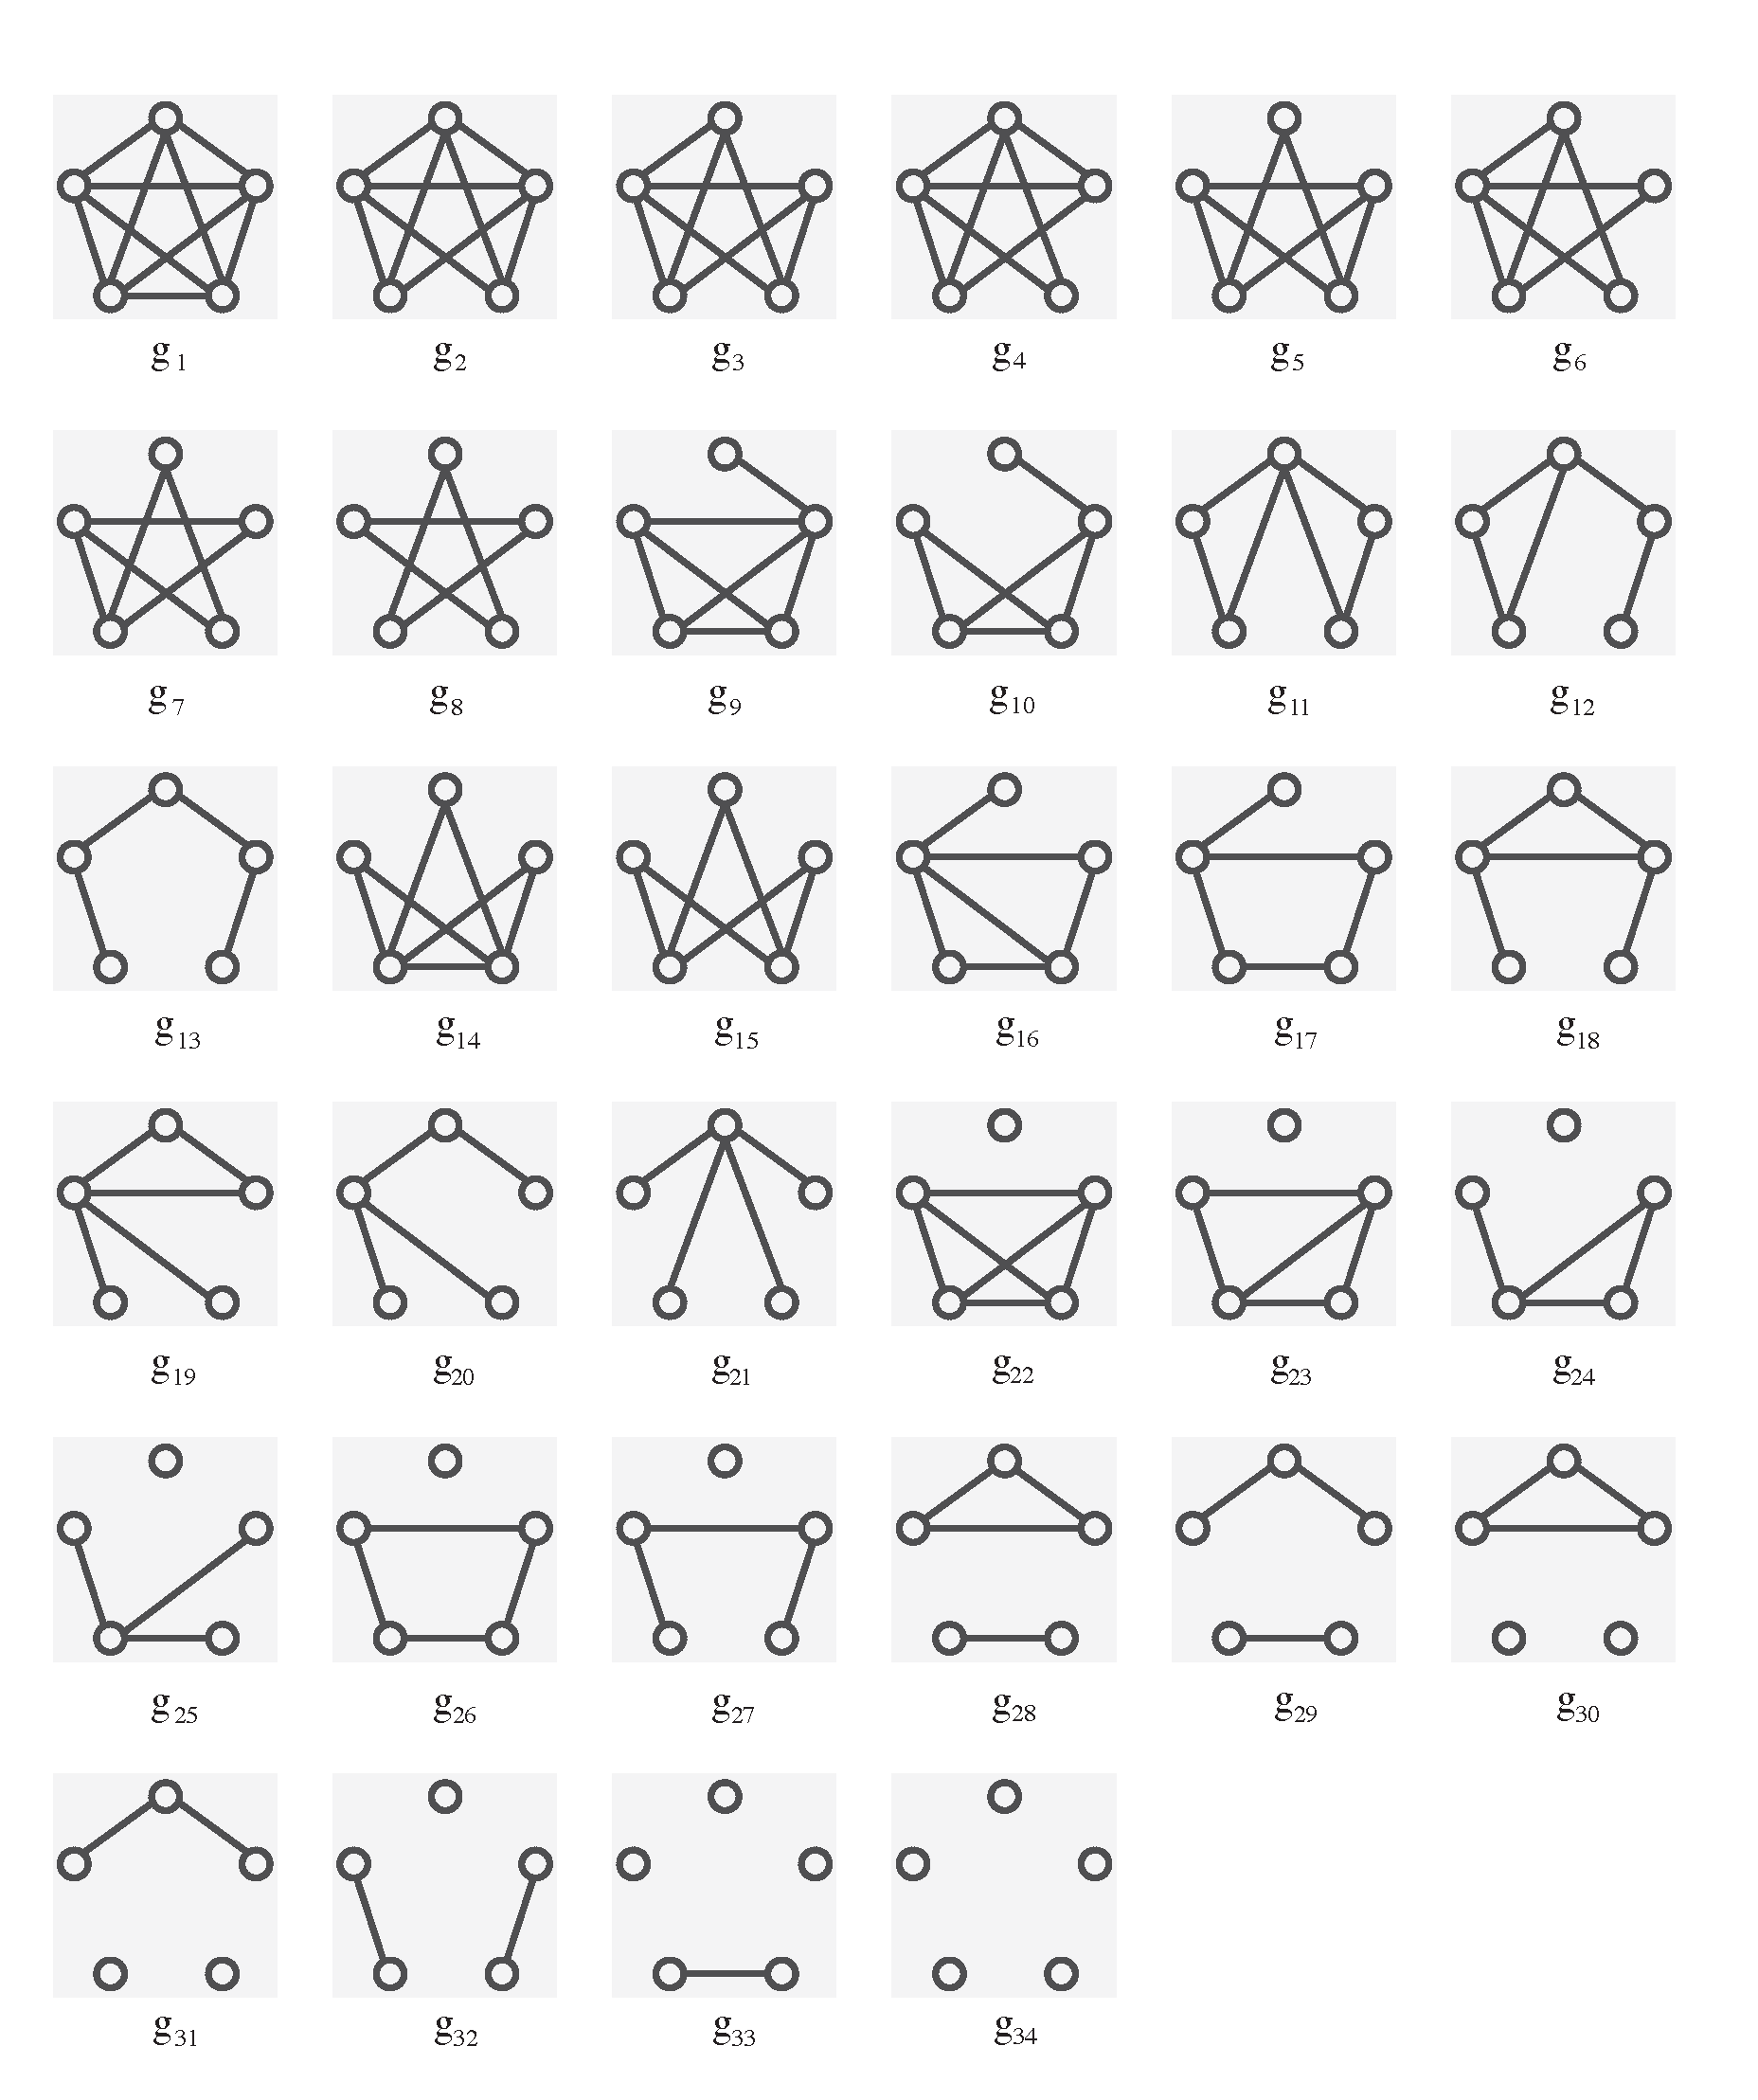
\includegraphics[width =\linewidth]{5graphlets.pdf}
\caption{Graphlets der Gr\"o"se 5 (\textit{Shervashidze et al.})}
\label{fig:5graphlets}
\end{figure}


%TODO: UML Diagramm so, konvertieren, dass es eine Bounding Box hat und wieder einf\"ugen


\section{Literaturverzeichnis}


\bibliographystyle{plain}
\bibliography{literatur}



\end{document}